\section{Motivation}
\begin{frame}[c]{Motivation}
\begin{tcolorbox}[colback=TUMBlueLighter,title=\dom]
    \begin{tabularx}{1.0\textwidth}{>{\hsize=0.30\hsize}X>{\hsize=0.8\hsize}X}
        \textbf{Input} & Graph $G = (V, E)$, $k \in \mathbb{N}$\\
        \textbf{Question} & Exists {$D \subseteq V$} with $|D| \leq k$ such that ${N[D] = V}$? \\
    \end{tabularx}
\end{tcolorbox}

\begin{itemize}
\pause \item The domination number is the minimum cardinality of a ds of $G$, denotes as $\gamma(G)$
\pause \item \textbf{Observation:} In connected $G$ every $v\in D$ has another $z \in D$ with $d(v,z) \leq 3$.
\end{itemize}

\end{frame}

\begin{frame}[c]{Motivation}
\begin{tcolorbox}[colback=TUMBlueLighter,title=\tdom]
    \begin{tabularx}{1.0\textwidth}{>{\hsize=0.30\hsize}X>{\hsize=0.8\hsize}X}
        \textbf{Input} & Graph $G = (V, E)$, $k \in \mathbb{N}$\\
        \textbf{Question} & Exists $D \subseteq V$ with $|D| \leq k$ such that \\ 
       &  $\forall d_1 \in X :\exists d_2 \in D \setminus \{d_1\}$ with ${d(d_1, d_2) \leq 1}$? \\
    \end{tabularx}
\end{tcolorbox}

\begin{itemize}
 \pause \item The total domination number is the minimum cardinality of a tds of $G$, denoted as $\gamma_t(G)$.
 \pause \item We say $d_1$ witnesses $d_2$ (and vice versa)
\end{itemize}

\end{frame}

\begin{frame}[c]{Motivation}
\begin{tcolorbox}[colback=TUMBlueLighter,title=\sdom]
    \begin{tabularx}{1.0\textwidth}{>{\hsize=0.30\hsize}X>{\hsize=0.8\hsize}X}
        \textbf{Input}    & Graph $G = (V, E)$, $k \in \mathbb{N}$\\
        \textbf{Question} & Exists $D \subseteq V$ with $|D| \leq k$ such that  \\
        & $\forall d_1 \in X :\exists d_2 \in D \setminus \{d_1\}$ with ${d(d_1, d_2) \leq 2}$? \\
    \end{tabularx}
\end{tcolorbox}

\begin{itemize}
    \pause \item The semitotal domination number is the minimum cardinality of an sds of $G$, denoted as $\gamma_{2t}(G)$.
    \pause \item \textbf{Observation}: $\gamma(G) \leq  \mathbf{\gamma_{2t}(G)}  \leq \gamma{t}(G)$
    \pause \item We say $d_1$ witnesses $d_2$ (and vice versa)
\end{itemize}
\end{frame}

\begin{frame}[c]{Example: $\gamma(G) < \mathbf{\gamma_{2t}(G)} < \gamma_t(G)$}
\begin{figure}[!ht]
    \resizebox{0.95\textwidth}{!}{
         \tikzfig{../thesis/fig/tikz/ds-examples}
    }
    \end{figure}
\end{frame}

\section{Theory}
\begin{frame}[c]{Parameterized Complexity}
    \begin{itemize}
        \pause \item NP-hard? We expect problem to be  \textbf{at least} exponential \\
         % \item Can we do something? Yes! \textbf{Parameterized Complexity} \\
        \pause \item \textbf{Idea:~} Limit combinatorial explosion to some aspect of the problem\\
        \pause \item \textbf{Goal: } Find an algorithm running in time $\mathcal{O}(f(k) \cdot n^c)$ for \textbf{some} parameter k
        \pause \item In this work: by solution size
        \pause \item \textbf{Techniques: } Kernelization, Bounded Search Trees, ... 
    \end{itemize}

If possible, the problem is \textbf{fixed-parameter tractable}.

\end{frame}

\subsection{Intractability}
\begin{frame}[c]{Fixed-Parameter Intractability}
    \begin{itemize}
       \pause \item  Class NP corresponds to whole hierarchy $W[i]$ in parameterized setting.
       \pause \item Problems at least $W[1]$-hard considered \textbf{fixed-parameter intractable}
       \pause \item \dom is $W[2]$-complete
       \pause \item \textbf{Tool for Proving Hardness}: FPT Reductions, preserving the parameter
    \end{itemize}
\end{frame}

\begin{frame}[c]{Complexity Comparison}

    \begin{table}
    \centering
    \resizebox{0.8\textwidth}{!}{
    \begin{tabularx}{1.5\textwidth}{lllllll}

        \arrayrulecolor{TUMBlue}\toprule

        \textbf{Graph Class}                  & \multicolumn{2}{c}{\textbf{\dom}}                       & \multicolumn{2}{c}{\textbf{\sdom}}           & \multicolumn{2}{c}{\textbf{\tdom}}                                                                                                                                \\
        \cmidrule(lr){2-3} \cmidrule(lr){4-5} \cmidrule(lr){6-7}    & classical                                               & Parameterized                                & classical                                               & Parameterized              & classical                                    & Parameterized               \\
        bipartite                             & \NPcs~\cite{Bertossi1984}                               & \WTWOhs~\cite{Raman2008}                                      & \NPcs~\cite{Henning2019}                                & \WTWOhs (this)             & \NPcs~\cite{Pfaff1983}                       & \WTWOhs (cite!)                             \\        
        line graph of bipartite               & \NPcs~\cite{Korobitsin1992}                             & ? & \NPcs~\cite{Galby2020}                                  &     ?         (?)              & \NPcs~\cite{McRae1995}                       &  ?                            \\
        
        circle                                & \NPcs~\cite{Keil1993}                                   & \WONEhs~\cite{Bousquet2012}                  & \NPcs~\cite{Kloks2021}                                  & ? (?)  & \NPcs~\cite{McRae1995}                       & \WONEhs~\cite{Bousquet2012} \\
        
        chordal                               & \NPcs~\cite{Booth1982}                                  & \WTWOhs~\cite{Raman2008}                     & \NPcs~\cite{Henning2019}                                & \WTWOhs (this)               & \NPcs~\cite{Laskar1983}                      & \WONEhs~\cite{Chang1998} by \textit{split}                            \\
        
        $s$-chordal , $s > 3$                          & \NPcs~\cite{Liu2011}                                    & \WTWOhs~\cite{Liu2011}                       & ? (?)                                                     & ? (?)                         & \NPcs~\cite{Liu2011}                         & \WONEhs~\cite{Liu2011}      \\
        
        split                                 & \NPcs~\cite{Bertossi1984}                               & \WTWOhs~\cite{Raman2008}         & \NPcs~\cite{Henning2019}                                & \WTWOhs \textbf{this}             & \NPcs~\cite{Laskar1983}                      & \WONEhs~\cite{Chang1998}    \\
        
        3-claw-free                           & \NPcs~\cite{Cygan2011}                                  & \FPTt~\cite{Cygan2011}                        & Prob. Unk                                               & Prob. Unk                  & \NPcs~\cite{McRae1995}                       & Unknown                     \\
        
        $t$-claw-free, $t>3$                  & \NPcs~\cite{Cygan2011}                                  & \WTWOhs~\cite{Cygan2011}                     & Prob. Unknown                                           & Unknown                    & \NPcs~\cite{McRae1995}                       & Prob. Unknown               \\
        
        chordal bipartite                     & \NPcs~\cite{Mueller1987}                                & ? (?)                                & \NPcs~\cite{Henning2019}                                & ?                      & \multicolumn{2}{c}{\Ptt~\cite{Damaschke1990}}                               \\
        
        planar                                & \NPcs (Sources!)                                        & \FPTt~\cite{Alber2004}                        & \NPcs                                                   & \FPT \textbf{(this)}                       & \NPcs                                        & \FPTt~\cite{Garnero2018}     \\
        
        undirected path                                & \NPcs~\cite{Booth1982}                                   & \FPTt~\cite{Figueiredo2022} & \NPcs~\cite{Henning2022}  & ?                     & \NPcs~\cite{Lan2014}                         & ?                     \\
        % 2022 paper for DS proved it not for TDS, so whp. not known for TDS
%
        dually chordal                        & \multicolumn{2}{c}{\Ptt~\cite{Brandstaedt1998} }         & \multicolumn{2}{c}{? (attempted~\cite{Galby2020})} &                           \multicolumn{2}{c}{\Ptt~\cite{Kratsch1997}}                                                                            \\
        
        strongly chordal                      & \multicolumn{2}{c}{\Ptt~\cite{Farber1984} }            & \multicolumn{2}{c}{\Ptt~\cite{Tripathi2021}}  & \NPcs~\cite{Farber1984}                                 &                                                                                                         \\
        
        AT-free                               & \multicolumn{2}{c}{\Ptt~\cite{Kratsch2000}}              & \multicolumn{2}{c}{\Ptt~\cite{Kloks2021} }    & \multicolumn{2}{c}{\Ptt~\cite{Kratsch2000}}                                                                                                                        \\
        
        tolerance                             & \multicolumn{2}{c}{\Ptt~\cite{Giannopoulou2016}}                         & \multicolumn{2}{c}{?}                                                  & \multicolumn{2}{c}{?}                                                                    \\
        
       block                        &                                                      \multicolumn{2}{c}{\Ptt~\cite{Farber1984} }                                          & \multicolumn{2}{c}{\Ptt~\cite{Henning2022}}              & \multicolumn{2}{c}{\Ptt~\cite{Chang1989}}                                                                       \\
        
        interval                  & \multicolumn{2}{c}{\Ptt~\cite{Chang1998a}}                                          & \multicolumn{2}{c}{\Ptt~\cite{Pradhan2021}} &                                         \multicolumn{2}{c}{\Ptt~\cite{Bertossi1986}}                       \\

        \midrule
        bounded clique-width                  & \multicolumn{2}{c}{\Ptt~\cite{Courcelle1990}}            & \multicolumn{2}{c}{\Ptt~\cite{Courcelle1990}} & \multicolumn{2}{c}{\Ptt~\cite{Courcelle1990}}                                                                                                                      \\
        
        bounded mim-width                     & \multicolumn{2}{c}{\Ptt~\cite{Belmonte2011,BuiXuan2013}} & \multicolumn{2}{c}{\Ptt~\cite{Galby2020}}     & \multicolumn{2}{c}{\Ptt~\cite{Belmonte2011,BuiXuan2013}}                                                                                                           \\
        \midrule
    \end{tabularx}
        }
\end{table}
\end{frame}

\begin{frame}[c]{Status \sdom}
 \begin{figure}
    \centering

    \makeatletter
    \resizebox{0.7\textwidth}{!}{
        

\tikzset{every picture/.style={line width=0.75pt}} %set default line width to 0.75pt        

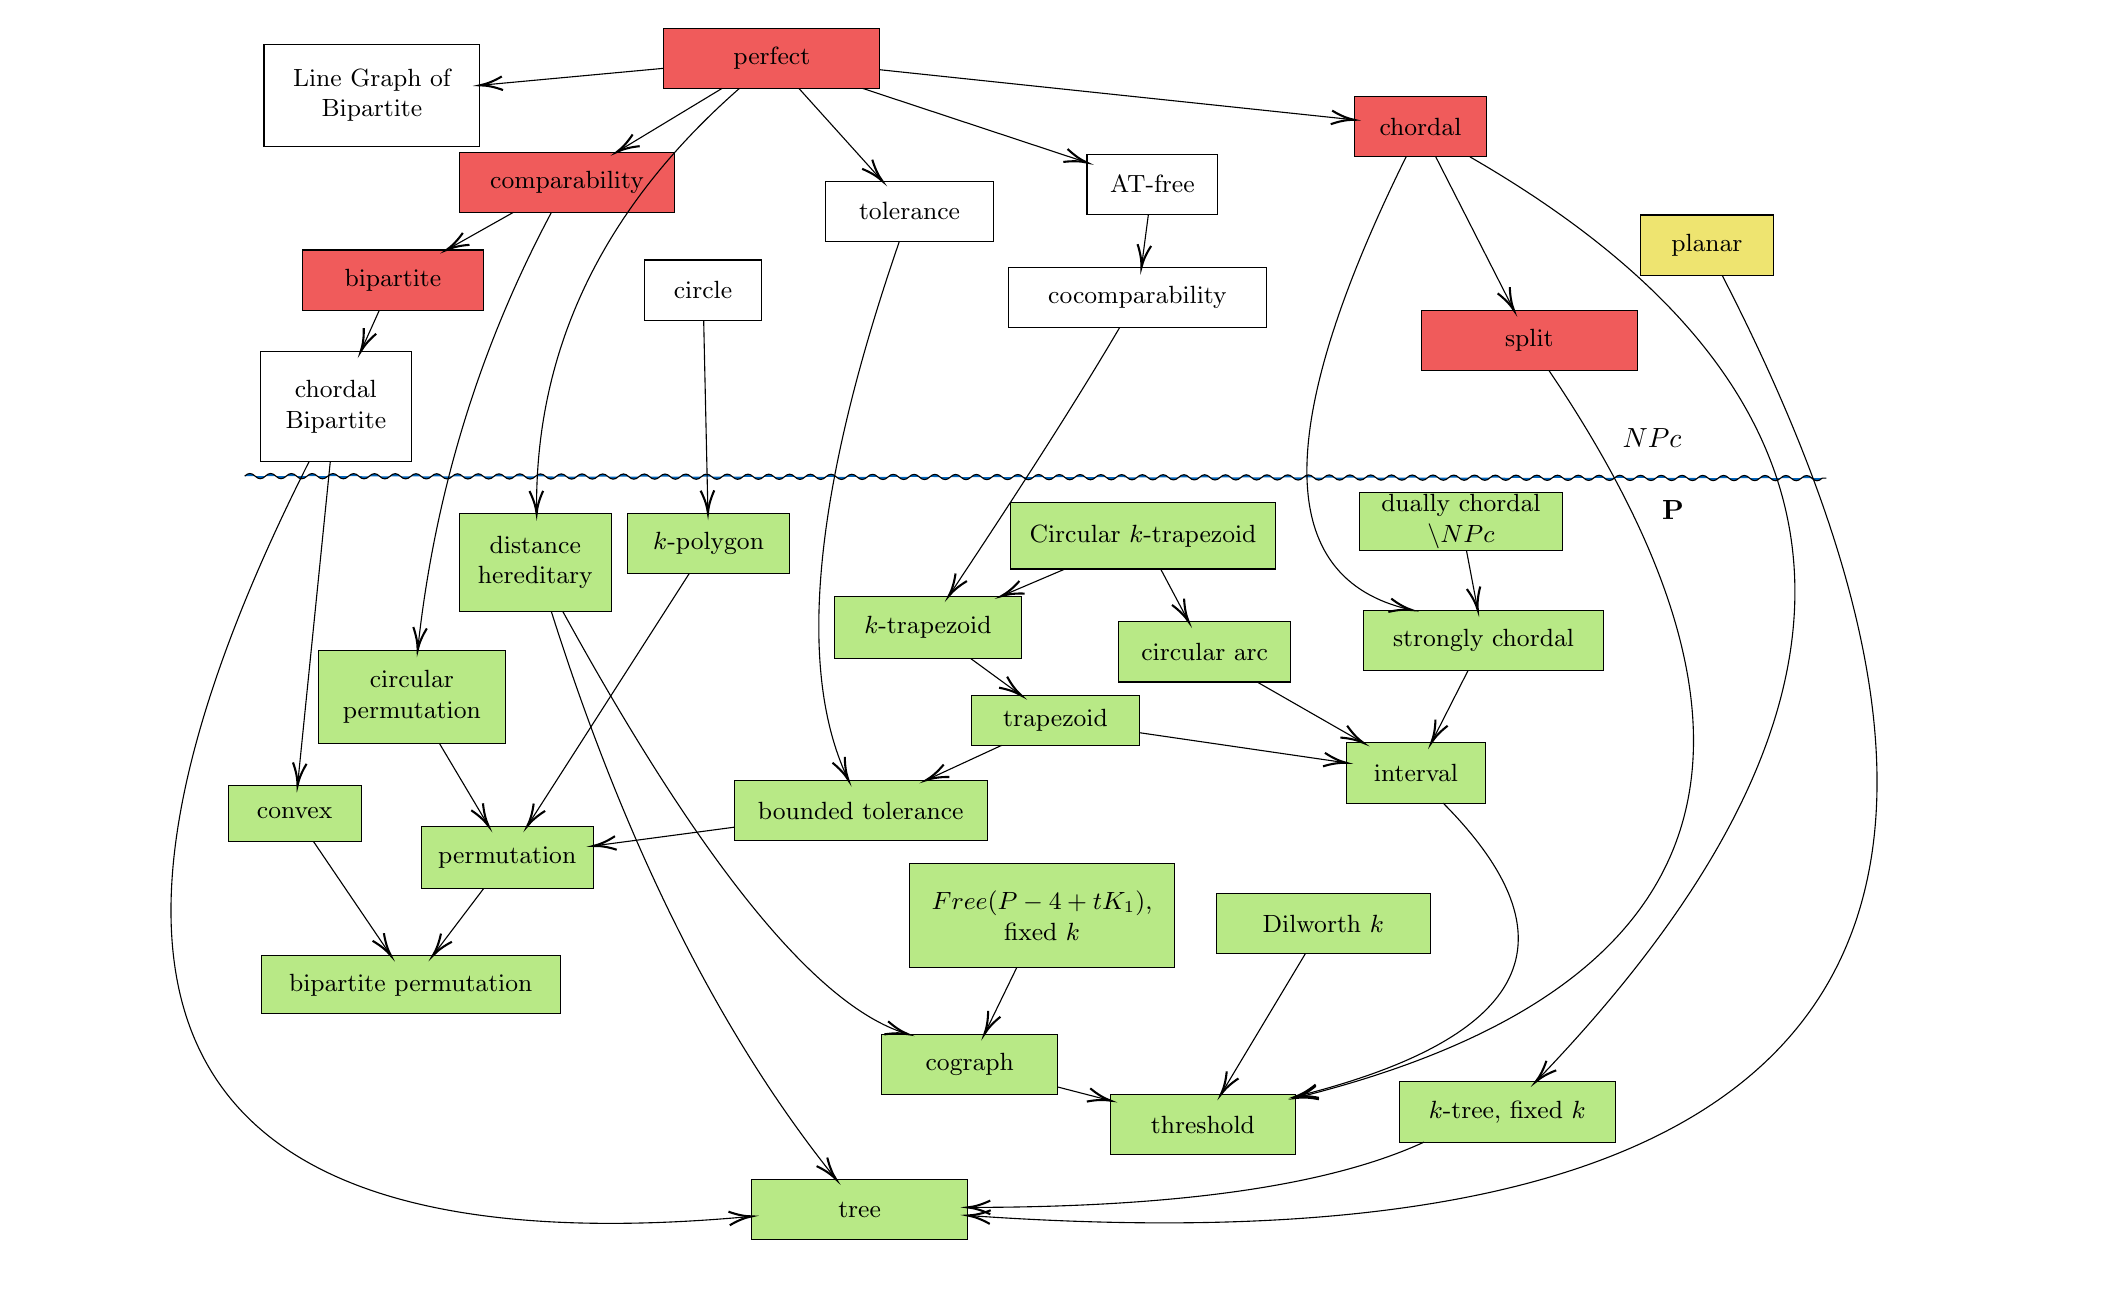
\begin{tikzpicture}[x=0.75pt,y=0.75pt,yscale=-1,xscale=1]
%uncomment if require: \path (0,617); %set diagram left start at 0, and has height of 617

%Straight Lines [id:da6521298779049807] 
\draw [fill={rgb, 255:red, 0; green, 101; blue, 189 }  ,fill opacity=1 ]   (0.4,215.38) .. controls (2.07,213.71) and (3.73,213.71) .. (5.4,215.38) .. controls (7.07,217.05) and (8.73,217.05) .. (10.4,215.39) .. controls (12.07,213.72) and (13.73,213.72) .. (15.4,215.39) .. controls (17.07,217.06) and (18.73,217.06) .. (20.4,215.4) .. controls (22.07,213.74) and (23.73,213.74) .. (25.4,215.41) .. controls (27.07,217.08) and (28.73,217.08) .. (30.4,215.41) .. controls (32.07,213.75) and (33.73,213.75) .. (35.4,215.42) .. controls (37.07,217.09) and (38.73,217.09) .. (40.4,215.43) .. controls (42.07,213.76) and (43.73,213.76) .. (45.4,215.43) .. controls (47.07,217.1) and (48.73,217.1) .. (50.4,215.44) .. controls (52.07,213.78) and (53.73,213.78) .. (55.4,215.45) .. controls (57.07,217.12) and (58.73,217.12) .. (60.4,215.45) .. controls (62.07,213.79) and (63.73,213.79) .. (65.4,215.46) .. controls (67.07,217.13) and (68.73,217.13) .. (70.4,215.47) .. controls (72.07,213.8) and (73.73,213.8) .. (75.4,215.47) .. controls (77.07,217.14) and (78.73,217.14) .. (80.4,215.48) .. controls (82.07,213.82) and (83.73,213.82) .. (85.4,215.49) .. controls (87.07,217.16) and (88.73,217.16) .. (90.4,215.49) .. controls (92.07,213.83) and (93.73,213.83) .. (95.4,215.5) .. controls (97.07,217.17) and (98.73,217.17) .. (100.4,215.51) .. controls (102.07,213.84) and (103.73,213.84) .. (105.4,215.51) .. controls (107.07,217.18) and (108.73,217.18) .. (110.4,215.52) .. controls (112.07,213.86) and (113.73,213.86) .. (115.4,215.53) .. controls (117.07,217.2) and (118.73,217.2) .. (120.4,215.53) .. controls (122.07,213.87) and (123.73,213.87) .. (125.4,215.54) .. controls (127.07,217.21) and (128.73,217.21) .. (130.4,215.55) .. controls (132.07,213.88) and (133.73,213.88) .. (135.4,215.55) .. controls (137.07,217.22) and (138.73,217.22) .. (140.4,215.56) .. controls (142.07,213.9) and (143.73,213.9) .. (145.4,215.57) .. controls (147.07,217.24) and (148.73,217.24) .. (150.4,215.57) .. controls (152.07,213.91) and (153.73,213.91) .. (155.4,215.58) .. controls (157.07,217.25) and (158.73,217.25) .. (160.4,215.58) .. controls (162.07,213.92) and (163.73,213.92) .. (165.4,215.59) .. controls (167.07,217.26) and (168.73,217.26) .. (170.4,215.6) .. controls (172.07,213.93) and (173.73,213.93) .. (175.4,215.6) .. controls (177.07,217.27) and (178.73,217.27) .. (180.4,215.61) .. controls (182.07,213.95) and (183.73,213.95) .. (185.4,215.62) .. controls (187.07,217.29) and (188.73,217.29) .. (190.4,215.62) .. controls (192.07,213.96) and (193.73,213.96) .. (195.4,215.63) .. controls (197.07,217.3) and (198.73,217.3) .. (200.4,215.64) .. controls (202.07,213.97) and (203.73,213.97) .. (205.4,215.64) .. controls (207.07,217.31) and (208.73,217.31) .. (210.4,215.65) .. controls (212.07,213.99) and (213.73,213.99) .. (215.4,215.66) .. controls (217.07,217.33) and (218.73,217.33) .. (220.4,215.66) .. controls (222.07,214) and (223.73,214) .. (225.4,215.67) .. controls (227.07,217.34) and (228.73,217.34) .. (230.4,215.68) .. controls (232.07,214.01) and (233.73,214.01) .. (235.4,215.68) .. controls (237.07,217.35) and (238.73,217.35) .. (240.4,215.69) .. controls (242.07,214.03) and (243.73,214.03) .. (245.4,215.7) .. controls (247.07,217.37) and (248.73,217.37) .. (250.4,215.7) .. controls (252.07,214.04) and (253.73,214.04) .. (255.4,215.71) .. controls (257.07,217.38) and (258.73,217.38) .. (260.4,215.72) .. controls (262.07,214.05) and (263.73,214.05) .. (265.4,215.72) .. controls (267.07,217.39) and (268.73,217.39) .. (270.4,215.73) .. controls (272.07,214.07) and (273.73,214.07) .. (275.4,215.74) .. controls (277.07,217.41) and (278.73,217.41) .. (280.4,215.74) .. controls (282.07,214.08) and (283.73,214.08) .. (285.4,215.75) .. controls (287.07,217.42) and (288.73,217.42) .. (290.4,215.76) .. controls (292.07,214.09) and (293.73,214.09) .. (295.4,215.76) .. controls (297.07,217.43) and (298.73,217.43) .. (300.4,215.77) .. controls (302.07,214.11) and (303.73,214.11) .. (305.4,215.78) .. controls (307.07,217.45) and (308.73,217.45) .. (310.4,215.78) .. controls (312.07,214.12) and (313.73,214.12) .. (315.4,215.79) .. controls (317.07,217.46) and (318.73,217.46) .. (320.4,215.79) .. controls (322.07,214.13) and (323.73,214.13) .. (325.4,215.8) .. controls (327.07,217.47) and (328.73,217.47) .. (330.4,215.81) .. controls (332.07,214.14) and (333.73,214.14) .. (335.4,215.81) .. controls (337.07,217.48) and (338.73,217.48) .. (340.4,215.82) .. controls (342.07,214.16) and (343.73,214.16) .. (345.4,215.83) .. controls (347.07,217.5) and (348.73,217.5) .. (350.4,215.83) .. controls (352.07,214.17) and (353.73,214.17) .. (355.4,215.84) .. controls (357.07,217.51) and (358.73,217.51) .. (360.4,215.85) .. controls (362.07,214.18) and (363.73,214.18) .. (365.4,215.85) .. controls (367.07,217.52) and (368.73,217.52) .. (370.4,215.86) .. controls (372.07,214.2) and (373.73,214.2) .. (375.4,215.87) .. controls (377.07,217.54) and (378.73,217.54) .. (380.4,215.87) .. controls (382.07,214.21) and (383.73,214.21) .. (385.4,215.88) .. controls (387.07,217.55) and (388.73,217.55) .. (390.4,215.89) .. controls (392.07,214.22) and (393.73,214.22) .. (395.4,215.89) .. controls (397.07,217.56) and (398.73,217.56) .. (400.4,215.9) .. controls (402.07,214.24) and (403.73,214.24) .. (405.4,215.91) .. controls (407.07,217.58) and (408.73,217.58) .. (410.4,215.91) .. controls (412.07,214.25) and (413.73,214.25) .. (415.4,215.92) .. controls (417.07,217.59) and (418.73,217.59) .. (420.4,215.93) .. controls (422.07,214.26) and (423.73,214.26) .. (425.4,215.93) .. controls (427.07,217.6) and (428.73,217.6) .. (430.4,215.94) .. controls (432.07,214.28) and (433.73,214.28) .. (435.4,215.95) .. controls (437.07,217.62) and (438.73,217.62) .. (440.4,215.95) .. controls (442.07,214.29) and (443.73,214.29) .. (445.4,215.96) .. controls (447.07,217.63) and (448.73,217.63) .. (450.4,215.97) .. controls (452.07,214.3) and (453.73,214.3) .. (455.4,215.97) .. controls (457.07,217.64) and (458.73,217.64) .. (460.4,215.98) .. controls (462.07,214.32) and (463.73,214.32) .. (465.4,215.99) .. controls (467.07,217.66) and (468.73,217.66) .. (470.4,215.99) .. controls (472.07,214.33) and (473.73,214.33) .. (475.4,216) .. controls (477.07,217.67) and (478.73,217.67) .. (480.4,216) .. controls (482.07,214.34) and (483.73,214.34) .. (485.4,216.01) .. controls (487.07,217.68) and (488.73,217.68) .. (490.4,216.02) .. controls (492.07,214.35) and (493.73,214.35) .. (495.4,216.02) .. controls (497.07,217.69) and (498.73,217.69) .. (500.4,216.03) .. controls (502.07,214.37) and (503.73,214.37) .. (505.4,216.04) .. controls (507.07,217.71) and (508.73,217.71) .. (510.4,216.04) .. controls (512.07,214.38) and (513.73,214.38) .. (515.4,216.05) .. controls (517.07,217.72) and (518.73,217.72) .. (520.4,216.06) .. controls (522.07,214.39) and (523.73,214.39) .. (525.4,216.06) .. controls (527.07,217.73) and (528.73,217.73) .. (530.4,216.07) .. controls (532.07,214.41) and (533.73,214.41) .. (535.4,216.08) .. controls (537.07,217.75) and (538.73,217.75) .. (540.4,216.08) .. controls (542.07,214.42) and (543.73,214.42) .. (545.4,216.09) .. controls (547.07,217.76) and (548.73,217.76) .. (550.4,216.1) .. controls (552.07,214.43) and (553.73,214.43) .. (555.4,216.1) .. controls (557.07,217.77) and (558.73,217.77) .. (560.4,216.11) .. controls (562.07,214.45) and (563.73,214.45) .. (565.4,216.12) .. controls (567.07,217.79) and (568.73,217.79) .. (570.4,216.12) .. controls (572.07,214.46) and (573.73,214.46) .. (575.4,216.13) .. controls (577.07,217.8) and (578.73,217.8) .. (580.4,216.14) .. controls (582.07,214.47) and (583.73,214.47) .. (585.4,216.14) .. controls (587.07,217.81) and (588.73,217.81) .. (590.4,216.15) .. controls (592.07,214.49) and (593.73,214.49) .. (595.4,216.16) .. controls (597.07,217.83) and (598.73,217.83) .. (600.4,216.16) .. controls (602.07,214.5) and (603.73,214.5) .. (605.4,216.17) .. controls (607.07,217.84) and (608.73,217.84) .. (610.4,216.18) .. controls (612.07,214.51) and (613.73,214.51) .. (615.4,216.18) .. controls (617.07,217.85) and (618.73,217.85) .. (620.4,216.19) .. controls (622.07,214.53) and (623.73,214.53) .. (625.4,216.2) .. controls (627.07,217.87) and (628.73,217.87) .. (630.4,216.2) .. controls (632.07,214.54) and (633.73,214.54) .. (635.4,216.21) .. controls (637.07,217.88) and (638.73,217.88) .. (640.4,216.21) .. controls (642.07,214.55) and (643.73,214.55) .. (645.4,216.22) .. controls (647.07,217.89) and (648.73,217.89) .. (650.4,216.23) .. controls (652.07,214.56) and (653.73,214.56) .. (655.4,216.23) .. controls (657.07,217.9) and (658.73,217.9) .. (660.4,216.24) .. controls (662.07,214.58) and (663.73,214.58) .. (665.4,216.25) .. controls (667.07,217.92) and (668.73,217.92) .. (670.4,216.25) .. controls (672.07,214.59) and (673.73,214.59) .. (675.4,216.26) .. controls (677.07,217.93) and (678.73,217.93) .. (680.4,216.27) .. controls (682.07,214.6) and (683.73,214.6) .. (685.4,216.27) .. controls (687.07,217.94) and (688.73,217.94) .. (690.4,216.28) .. controls (692.07,214.62) and (693.73,214.62) .. (695.4,216.29) .. controls (697.07,217.96) and (698.73,217.96) .. (700.4,216.29) .. controls (702.07,214.63) and (703.73,214.63) .. (705.4,216.3) .. controls (707.07,217.97) and (708.73,217.97) .. (710.4,216.31) .. controls (712.07,214.64) and (713.73,214.64) .. (715.4,216.31) .. controls (717.07,217.98) and (718.73,217.98) .. (720.4,216.32) .. controls (722.07,214.66) and (723.73,214.66) .. (725.4,216.33) .. controls (727.07,218) and (728.73,218) .. (730.4,216.33) .. controls (732.07,214.67) and (733.73,214.67) .. (735.4,216.34) .. controls (737.07,218.01) and (738.73,218.01) .. (740.4,216.35) .. controls (742.07,214.68) and (743.73,214.68) .. (745.4,216.35) .. controls (747.07,218.02) and (748.73,218.02) .. (750.4,216.36) .. controls (752.07,214.7) and (753.73,214.7) .. (755.4,216.37) .. controls (757.07,218.04) and (758.73,218.04) .. (760.4,216.37) -- (762.4,216.38) -- (762.4,216.38) ;

% Text Node
\draw  [fill={rgb, 255:red, 233; green, 17; blue, 17 }  ,fill opacity=0.69 ]  (202.33,-0.4) -- (306.33,-0.4) -- (306.33,28.6) -- (202.33,28.6) -- cycle  ;
\draw (254.33,14.1) node  [font=\small] [align=left] {\begin{minipage}[lt]{68pt}\setlength\topsep{0pt}
\begin{center}
perfect
\end{center}

\end{minipage}};
% Text Node
\draw    (9.67,7.42) -- (113.67,7.42) -- (113.67,56.42) -- (9.67,56.42) -- cycle  ;
\draw (61.67,31.92) node  [font=\small] [align=left] {\begin{minipage}[lt]{68pt}\setlength\topsep{0pt}
\begin{center}
Line Graph of Bipartite
\end{center}

\end{minipage}};
% Text Node
\draw  [fill={rgb, 255:red, 233; green, 17; blue, 17 }  ,fill opacity=0.69 ]  (103.67,59.27) -- (207.67,59.27) -- (207.67,88.27) -- (103.67,88.27) -- cycle  ;
\draw (155.67,73.77) node  [font=\small] [align=left] {\begin{minipage}[lt]{68pt}\setlength\topsep{0pt}
\begin{center}
comparability
\end{center}

\end{minipage}};
% Text Node
\draw    (280.2,73.27) -- (361.2,73.27) -- (361.2,102.27) -- (280.2,102.27) -- cycle  ;
\draw (320.7,87.77) node  [font=\small] [align=left] {\begin{minipage}[lt]{52.63pt}\setlength\topsep{0pt}
\begin{center}
tolerance
\end{center}

\end{minipage}};
% Text Node
\draw    (406.2,60.27) -- (469.2,60.27) -- (469.2,89.27) -- (406.2,89.27) -- cycle  ;
\draw (437.7,74.77) node  [font=\small] [align=left] {\begin{minipage}[lt]{40.39pt}\setlength\topsep{0pt}
\begin{center}
AT-free
\end{center}

\end{minipage}};
% Text Node
\draw  [fill={rgb, 255:red, 233; green, 17; blue, 17 }  ,fill opacity=0.69 ]  (534.87,32.6) -- (598.87,32.6) -- (598.87,61.6) -- (534.87,61.6) -- cycle  ;
\draw (566.87,47.1) node  [font=\small] [align=left] {\begin{minipage}[lt]{40.62pt}\setlength\topsep{0pt}
\begin{center}
chordal
\end{center}

\end{minipage}};
% Text Node
\draw  [fill={rgb, 255:red, 233; green, 17; blue, 17 }  ,fill opacity=0.69 ]  (567.33,135.6) -- (671.33,135.6) -- (671.33,164.6) -- (567.33,164.6) -- cycle  ;
\draw (619.33,150.1) node  [font=\small] [align=left] {\begin{minipage}[lt]{68pt}\setlength\topsep{0pt}
\begin{center}
split
\end{center}

\end{minipage}};
% Text Node
\draw  [fill={rgb, 255:red, 184; green, 233; blue, 134 }  ,fill opacity=1 ]  (556.67,507.27) -- (660.67,507.27) -- (660.67,536.27) -- (556.67,536.27) -- cycle  ;
\draw (608.67,521.77) node  [font=\small] [align=left] {\begin{minipage}[lt]{68pt}\setlength\topsep{0pt}
\begin{center}
$\displaystyle k$-tree, fixed $\displaystyle k$
\end{center}

\end{minipage}};
% Text Node
\draw    (368.5,114.93) -- (492.5,114.93) -- (492.5,143.93) -- (368.5,143.93) -- cycle  ;
\draw (430.5,129.43) node  [font=\small] [align=left] {\begin{minipage}[lt]{81.83pt}\setlength\topsep{0pt}
\begin{center}
cocomparability
\end{center}

\end{minipage}};
% Text Node
\draw  [fill={rgb, 255:red, 184; green, 233; blue, 134 }  ,fill opacity=1 ]  (244.67,554.27) -- (348.67,554.27) -- (348.67,583.27) -- (244.67,583.27) -- cycle  ;
\draw (296.67,568.77) node  [font=\small] [align=left] {\begin{minipage}[lt]{68pt}\setlength\topsep{0pt}
\begin{center}
tree
\end{center}

\end{minipage}};
% Text Node
\draw    (193.2,111.27) -- (249.2,111.27) -- (249.2,140.27) -- (193.2,140.27) -- cycle  ;
\draw (221.2,125.77) node  [font=\small] [align=left] {\begin{minipage}[lt]{35.63pt}\setlength\topsep{0pt}
\begin{center}
circle
\end{center}

\end{minipage}};
% Text Node
\draw    (7.8,155.42) -- (80.8,155.42) -- (80.8,208.42) -- (7.8,208.42) -- cycle  ;
\draw (44.3,181.92) node  [font=\small] [align=left] {\begin{minipage}[lt]{47.1pt}\setlength\topsep{0pt}
\begin{center}
chordal Bipartite
\end{center}

\end{minipage}};
% Text Node
\draw  [fill={rgb, 255:red, 233; green, 17; blue, 17 }  ,fill opacity=0.69 ]  (28.3,106.47) -- (115.3,106.47) -- (115.3,135.47) -- (28.3,135.47) -- cycle  ;
\draw (71.8,120.97) node  [font=\small] [align=left] {\begin{minipage}[lt]{56.39pt}\setlength\topsep{0pt}
\begin{center}
bipartite
\end{center}

\end{minipage}};
% Text Node
\draw  [fill={rgb, 255:red, 184; green, 233; blue, 134 }  ,fill opacity=1 ]  (369.2,228.15) -- (497.2,228.15) -- (497.2,260.15) -- (369.2,260.15) -- cycle  ;
\draw (433.2,244.15) node  [font=\small] [align=left] {\begin{minipage}[lt]{84.59pt}\setlength\topsep{0pt}
\begin{center}
Circular $\displaystyle k$-trapezoid
\end{center}

\end{minipage}};
% Text Node
\draw  [fill={rgb, 255:red, 184; green, 233; blue, 134 }  ,fill opacity=1 ]  (284.6,273.24) -- (374.6,273.24) -- (374.6,303.24) -- (284.6,303.24) -- cycle  ;
\draw (329.6,288.24) node  [font=\small] [align=left] {\begin{minipage}[lt]{58.21pt}\setlength\topsep{0pt}
\begin{center}
$\displaystyle k$-trapezoid
\end{center}

\end{minipage}};
% Text Node
\draw  [fill={rgb, 255:red, 184; green, 233; blue, 134 }  ,fill opacity=1 ]  (350.53,321.12) -- (431.53,321.12) -- (431.53,345.12) -- (350.53,345.12) -- cycle  ;
\draw (391.03,333.12) node  [font=\small] [align=left] {\begin{minipage}[lt]{52.18pt}\setlength\topsep{0pt}
\begin{center}
trapezoid
\end{center}

\end{minipage}};
% Text Node
\draw  [fill={rgb, 255:red, 184; green, 233; blue, 134 }  ,fill opacity=1 ]  (236.2,361.93) -- (358.2,361.93) -- (358.2,390.93) -- (236.2,390.93) -- cycle  ;
\draw (297.2,376.43) node  [font=\small] [align=left] {\begin{minipage}[lt]{80.51pt}\setlength\topsep{0pt}
\begin{center}
bounded tolerance
\end{center}

\end{minipage}};
% Text Node
\draw  [fill={rgb, 255:red, 184; green, 233; blue, 134 }  ,fill opacity=1 ]  (85.37,384.11) -- (168.37,384.11) -- (168.37,414.11) -- (85.37,414.11) -- cycle  ;
\draw (126.87,399.11) node  [font=\small] [align=left] {\begin{minipage}[lt]{53.77pt}\setlength\topsep{0pt}
\begin{center}
permutation
\end{center}

\end{minipage}};
% Text Node
\draw  [fill={rgb, 255:red, 184; green, 233; blue, 134 }  ,fill opacity=1 ]  (8.37,446.49) -- (152.37,446.49) -- (152.37,474.49) -- (8.37,474.49) -- cycle  ;
\draw (80.37,460.49) node  [font=\small] [align=left] {\begin{minipage}[lt]{95.25pt}\setlength\topsep{0pt}
\begin{center}
bipartite permutation
\end{center}

\end{minipage}};
% Text Node
\draw  [fill={rgb, 255:red, 184; green, 233; blue, 134 }  ,fill opacity=1 ]  (-7.53,364.57) -- (56.47,364.57) -- (56.47,391.57) -- (-7.53,391.57) -- cycle  ;
\draw (24.47,378.07) node  [font=\small] [align=left] {\begin{minipage}[lt]{40.53pt}\setlength\topsep{0pt}
\begin{center}
convex
\end{center}

\end{minipage}};
% Text Node
\draw  [fill={rgb, 255:red, 184; green, 233; blue, 134 }  ,fill opacity=1 ]  (531.2,343.93) -- (598.2,343.93) -- (598.2,372.93) -- (531.2,372.93) -- cycle  ;
\draw (564.7,358.43) node  [font=\small] [align=left] {\begin{minipage}[lt]{43.11pt}\setlength\topsep{0pt}
\begin{center}
interval
\end{center}

\end{minipage}};
% Text Node
\draw  [fill={rgb, 255:red, 184; green, 233; blue, 134 }  ,fill opacity=1 ]  (417.53,513.27) -- (506.53,513.27) -- (506.53,542.27) -- (417.53,542.27) -- cycle  ;
\draw (462.03,527.77) node  [font=\small] [align=left] {\begin{minipage}[lt]{57.62pt}\setlength\topsep{0pt}
\begin{center}
threshold
\end{center}

\end{minipage}};
% Text Node
\draw  [fill={rgb, 255:red, 184; green, 233; blue, 134 }  ,fill opacity=1 ]  (468.53,416.6) -- (571.53,416.6) -- (571.53,445.6) -- (468.53,445.6) -- cycle  ;
\draw (520.03,431.1) node  [font=\small] [align=left] {\begin{minipage}[lt]{67.14pt}\setlength\topsep{0pt}
\begin{center}
Dilworth $\displaystyle k$
\end{center}

\end{minipage}};
% Text Node
\draw  [fill={rgb, 255:red, 184; green, 233; blue, 134 }  ,fill opacity=1 ]  (307.2,484.27) -- (392.2,484.27) -- (392.2,513.27) -- (307.2,513.27) -- cycle  ;
\draw (349.7,498.77) node  [font=\small] [align=left] {\begin{minipage}[lt]{55.35pt}\setlength\topsep{0pt}
\begin{center}
cograph
\end{center}

\end{minipage}};
% Text Node
\draw  [fill={rgb, 255:red, 184; green, 233; blue, 134 }  ,fill opacity=1 ]  (421.4,285.6) -- (504.4,285.6) -- (504.4,314.6) -- (421.4,314.6) -- cycle  ;
\draw (462.9,300.1) node  [font=\small] [align=left] {\begin{minipage}[lt]{53.72pt}\setlength\topsep{0pt}
\begin{center}
circular arc
\end{center}

\end{minipage}};
% Text Node
\draw  [fill={rgb, 255:red, 184; green, 233; blue, 134 }  ,fill opacity=1 ]  (537.37,223.18) -- (635.37,223.18) -- (635.37,251.18) -- (537.37,251.18) -- cycle  ;
\draw (586.37,237.18) node  [font=\small] [align=left] {\begin{minipage}[lt]{63.97pt}\setlength\topsep{0pt}
\begin{center}
dually chordal $\displaystyle \backslash NPc$
\end{center}

\end{minipage}};
% Text Node
\draw  [fill={rgb, 255:red, 184; green, 233; blue, 134 }  ,fill opacity=1 ]  (539.23,279.93) -- (655.23,279.93) -- (655.23,308.93) -- (539.23,308.93) -- cycle  ;
\draw (597.23,294.43) node  [font=\small] [align=left] {\begin{minipage}[lt]{76.39pt}\setlength\topsep{0pt}
\begin{center}
strongly chordal
\end{center}

\end{minipage}};
% Text Node
\draw  [fill={rgb, 255:red, 184; green, 233; blue, 134 }  ,fill opacity=1 ]  (35.9,299.3) -- (125.9,299.3) -- (125.9,344.3) -- (35.9,344.3) -- cycle  ;
\draw (80.9,321.8) node  [font=\small] [align=left] {\begin{minipage}[lt]{58.34pt}\setlength\topsep{0pt}
\begin{center}
circular permutation
\end{center}

\end{minipage}};
% Text Node
\draw  [fill={rgb, 255:red, 184; green, 233; blue, 134 }  ,fill opacity=1 ]  (184.9,233.27) -- (262.9,233.27) -- (262.9,262.27) -- (184.9,262.27) -- cycle  ;
\draw (223.9,247.77) node  [font=\small] [align=left] {\begin{minipage}[lt]{50.18pt}\setlength\topsep{0pt}
\begin{center}
$\displaystyle k$-polygon
\end{center}

\end{minipage}};
% Text Node
\draw  [fill={rgb, 255:red, 184; green, 233; blue, 134 }  ,fill opacity=1 ]  (103.9,233.49) -- (176.9,233.49) -- (176.9,280.49) -- (103.9,280.49) -- cycle  ;
\draw (140.4,256.99) node  [font=\small] [align=left] {\begin{minipage}[lt]{46.78pt}\setlength\topsep{0pt}
\begin{center}
distance hereditary
\end{center}

\end{minipage}};
% Text Node
\draw  [fill={rgb, 255:red, 184; green, 233; blue, 134 }  ,fill opacity=1 ]  (320.53,402.14) -- (448.53,402.14) -- (448.53,452.14) -- (320.53,452.14) -- cycle  ;
\draw (384.53,427.14) node  [font=\small] [align=left] {\begin{minipage}[lt]{84.14pt}\setlength\topsep{0pt}
\begin{center}
$\displaystyle Free( P-4+tK_{1})$, fixed $\displaystyle k$
\end{center}

\end{minipage}};
% Text Node
\draw  [fill={rgb, 255:red, 230; green, 216; blue, 48 }  ,fill opacity=0.69 ]  (672.87,89.6) -- (736.87,89.6) -- (736.87,118.6) -- (672.87,118.6) -- cycle  ;
\draw (704.87,104.1) node  [font=\small] [align=left] {\begin{minipage}[lt]{40.62pt}\setlength\topsep{0pt}
\begin{center}
planar
\end{center}

\end{minipage}};
% Text Node
\draw (663,191) node [anchor=north west][inner sep=0.75pt]   [align=left] {$\displaystyle NPc$};
% Text Node
\draw (682,226) node [anchor=north west][inner sep=0.75pt]   [align=left] {\textbf{P}};
% Connection
\draw    (230.36,28.6) -- (181.36,58.23) ;
\draw [shift={(179.64,59.27)}, rotate = 328.84] [color={rgb, 255:red, 0; green, 0; blue, 0 }  ][line width=0.75]    (10.93,-3.29) .. controls (6.95,-1.4) and (3.31,-0.3) .. (0,0) .. controls (3.31,0.3) and (6.95,1.4) .. (10.93,3.29)   ;
% Connection
\draw    (267.4,28.6) -- (306.3,71.78) ;
\draw [shift={(307.64,73.27)}, rotate = 227.98] [color={rgb, 255:red, 0; green, 0; blue, 0 }  ][line width=0.75]    (10.93,-3.29) .. controls (6.95,-1.4) and (3.31,-0.3) .. (0,0) .. controls (3.31,0.3) and (6.95,1.4) .. (10.93,3.29)   ;
% Connection
\draw    (298.16,28.6) -- (404.3,63.72) ;
\draw [shift={(406.2,64.34)}, rotate = 198.31] [color={rgb, 255:red, 0; green, 0; blue, 0 }  ][line width=0.75]    (10.93,-3.29) .. controls (6.95,-1.4) and (3.31,-0.3) .. (0,0) .. controls (3.31,0.3) and (6.95,1.4) .. (10.93,3.29)   ;
% Connection
\draw    (306.33,19.59) -- (532.88,43.51) ;
\draw [shift={(534.87,43.72)}, rotate = 186.03] [color={rgb, 255:red, 0; green, 0; blue, 0 }  ][line width=0.75]    (10.93,-3.29) .. controls (6.95,-1.4) and (3.31,-0.3) .. (0,0) .. controls (3.31,0.3) and (6.95,1.4) .. (10.93,3.29)   ;
% Connection
\draw    (574.25,61.6) -- (611.04,133.82) ;
\draw [shift={(611.95,135.6)}, rotate = 243.01] [color={rgb, 255:red, 0; green, 0; blue, 0 }  ][line width=0.75]    (10.93,-3.29) .. controls (6.95,-1.4) and (3.31,-0.3) .. (0,0) .. controls (3.31,0.3) and (6.95,1.4) .. (10.93,3.29)   ;
% Connection
\draw    (590.74,61.6) .. controls (788.33,175.57) and (798.86,324.13) .. (622.31,507.27) ;
\draw [shift={(622.31,507.27)}, rotate = 313.95] [color={rgb, 255:red, 0; green, 0; blue, 0 }  ][line width=0.75]    (10.93,-3.29) .. controls (6.95,-1.4) and (3.31,-0.3) .. (0,0) .. controls (3.31,0.3) and (6.95,1.4) .. (10.93,3.29)   ;
% Connection
\draw    (435.79,89.27) -- (432.67,112.95) ;
\draw [shift={(432.41,114.93)}, rotate = 277.5] [color={rgb, 255:red, 0; green, 0; blue, 0 }  ][line width=0.75]    (10.93,-3.29) .. controls (6.95,-1.4) and (3.31,-0.3) .. (0,0) .. controls (3.31,0.3) and (6.95,1.4) .. (10.93,3.29)   ;
% Connection
\draw    (568.55,536.27) .. controls (523.28,557.16) and (450.49,567.64) .. (350.18,567.72) ;
\draw [shift={(348.67,567.72)}, rotate = 0.02] [color={rgb, 255:red, 0; green, 0; blue, 0 }  ][line width=0.75]    (10.93,-3.29) .. controls (6.95,-1.4) and (3.31,-0.3) .. (0,0) .. controls (3.31,0.3) and (6.95,1.4) .. (10.93,3.29)   ;
% Connection
\draw    (129.91,88.27) -- (99.3,105.49) ;
\draw [shift={(97.56,106.47)}, rotate = 330.62] [color={rgb, 255:red, 0; green, 0; blue, 0 }  ][line width=0.75]    (10.93,-3.29) .. controls (6.95,-1.4) and (3.31,-0.3) .. (0,0) .. controls (3.31,0.3) and (6.95,1.4) .. (10.93,3.29)   ;
% Connection
\draw    (65.26,135.47) -- (57.08,153.6) ;
\draw [shift={(56.26,155.42)}, rotate = 294.29] [color={rgb, 255:red, 0; green, 0; blue, 0 }  ][line width=0.75]    (10.93,-3.29) .. controls (6.95,-1.4) and (3.31,-0.3) .. (0,0) .. controls (3.31,0.3) and (6.95,1.4) .. (10.93,3.29)   ;
% Connection
\draw    (202.33,18.91) -- (115.66,26.93) ;
\draw [shift={(113.67,27.11)}, rotate = 354.72] [color={rgb, 255:red, 0; green, 0; blue, 0 }  ][line width=0.75]    (10.93,-3.29) .. controls (6.95,-1.4) and (3.31,-0.3) .. (0,0) .. controls (3.31,0.3) and (6.95,1.4) .. (10.93,3.29)   ;
% Connection
\draw    (395.6,260.15) -- (366.69,272.46) ;
\draw [shift={(364.85,273.24)}, rotate = 336.95] [color={rgb, 255:red, 0; green, 0; blue, 0 }  ][line width=0.75]    (10.93,-3.29) .. controls (6.95,-1.4) and (3.31,-0.3) .. (0,0) .. controls (3.31,0.3) and (6.95,1.4) .. (10.93,3.29)   ;
% Connection
\draw    (421.86,143.93) .. controls (403.18,175.74) and (376.1,218.31) .. (340.63,271.62) ;
\draw [shift={(339.55,273.24)}, rotate = 303.65] [color={rgb, 255:red, 0; green, 0; blue, 0 }  ][line width=0.75]    (10.93,-3.29) .. controls (6.95,-1.4) and (3.31,-0.3) .. (0,0) .. controls (3.31,0.3) and (6.95,1.4) .. (10.93,3.29)   ;
% Connection
\draw    (350.13,303.24) -- (372.99,319.94) ;
\draw [shift={(374.61,321.12)}, rotate = 216.15] [color={rgb, 255:red, 0; green, 0; blue, 0 }  ][line width=0.75]    (10.93,-3.29) .. controls (6.95,-1.4) and (3.31,-0.3) .. (0,0) .. controls (3.31,0.3) and (6.95,1.4) .. (10.93,3.29)   ;
% Connection
\draw    (365.04,345.12) -- (330.43,361.1) ;
\draw [shift={(328.61,361.93)}, rotate = 335.22] [color={rgb, 255:red, 0; green, 0; blue, 0 }  ][line width=0.75]    (10.93,-3.29) .. controls (6.95,-1.4) and (3.31,-0.3) .. (0,0) .. controls (3.31,0.3) and (6.95,1.4) .. (10.93,3.29)   ;
% Connection
\draw    (41.62,208.42) -- (26.03,362.59) ;
\draw [shift={(25.83,364.57)}, rotate = 275.77] [color={rgb, 255:red, 0; green, 0; blue, 0 }  ][line width=0.75]    (10.93,-3.29) .. controls (6.95,-1.4) and (3.31,-0.3) .. (0,0) .. controls (3.31,0.3) and (6.95,1.4) .. (10.93,3.29)   ;
% Connection
\draw [color={rgb, 255:red, 0; green, 0; blue, 0 }  ,draw opacity=1 ]   (33.62,391.57) -- (69.75,444.83) ;
\draw [shift={(70.87,446.49)}, rotate = 235.85] [color={rgb, 255:red, 0; green, 0; blue, 0 }  ,draw opacity=1 ][line width=0.75]    (10.93,-3.29) .. controls (6.95,-1.4) and (3.31,-0.3) .. (0,0) .. controls (3.31,0.3) and (6.95,1.4) .. (10.93,3.29)   ;
% Connection
\draw    (115.5,414.11) -- (92.18,444.89) ;
\draw [shift={(90.97,446.49)}, rotate = 307.15] [color={rgb, 255:red, 0; green, 0; blue, 0 }  ][line width=0.75]    (10.93,-3.29) .. controls (6.95,-1.4) and (3.31,-0.3) .. (0,0) .. controls (3.31,0.3) and (6.95,1.4) .. (10.93,3.29)   ;
% Connection
\draw    (236.2,384.55) -- (170.35,393.32) ;
\draw [shift={(168.37,393.58)}, rotate = 352.42] [color={rgb, 255:red, 0; green, 0; blue, 0 }  ][line width=0.75]    (10.93,-3.29) .. controls (6.95,-1.4) and (3.31,-0.3) .. (0,0) .. controls (3.31,0.3) and (6.95,1.4) .. (10.93,3.29)   ;
% Connection
\draw    (431.53,339.02) -- (529.22,353.26) ;
\draw [shift={(531.2,353.55)}, rotate = 188.29] [color={rgb, 255:red, 0; green, 0; blue, 0 }  ][line width=0.75]    (10.93,-3.29) .. controls (6.95,-1.4) and (3.31,-0.3) .. (0,0) .. controls (3.31,0.3) and (6.95,1.4) .. (10.93,3.29)   ;
% Connection
\draw    (577.8,372.93) .. controls (643.17,438.8) and (619.98,485.81) .. (508.22,513.97) ;
\draw [shift={(506.53,514.39)}, rotate = 346.05] [color={rgb, 255:red, 0; green, 0; blue, 0 }  ][line width=0.75]    (10.93,-3.29) .. controls (6.95,-1.4) and (3.31,-0.3) .. (0,0) .. controls (3.31,0.3) and (6.95,1.4) .. (10.93,3.29)   ;
% Connection
\draw    (392.2,509.74) -- (415.6,515.78) ;
\draw [shift={(417.53,516.28)}, rotate = 194.48] [color={rgb, 255:red, 0; green, 0; blue, 0 }  ][line width=0.75]    (10.93,-3.29) .. controls (6.95,-1.4) and (3.31,-0.3) .. (0,0) .. controls (3.31,0.3) and (6.95,1.4) .. (10.93,3.29)   ;
% Connection
\draw    (511.33,445.6) -- (471.76,511.55) ;
\draw [shift={(470.73,513.27)}, rotate = 300.96] [color={rgb, 255:red, 0; green, 0; blue, 0 }  ][line width=0.75]    (10.93,-3.29) .. controls (6.95,-1.4) and (3.31,-0.3) .. (0,0) .. controls (3.31,0.3) and (6.95,1.4) .. (10.93,3.29)   ;
% Connection
\draw    (628.84,164.6) .. controls (752.25,347.55) and (711.48,464.37) .. (506.53,515.04) ;
\draw [shift={(506.53,515.04)}, rotate = 346.11] [color={rgb, 255:red, 0; green, 0; blue, 0 }  ][line width=0.75]    (10.93,-3.29) .. controls (6.95,-1.4) and (3.31,-0.3) .. (0,0) .. controls (3.31,0.3) and (6.95,1.4) .. (10.93,3.29)   ;
% Connection
\draw    (488.2,314.6) -- (537.66,342.94) ;
\draw [shift={(539.4,343.93)}, rotate = 209.81] [color={rgb, 255:red, 0; green, 0; blue, 0 }  ][line width=0.75]    (10.93,-3.29) .. controls (6.95,-1.4) and (3.31,-0.3) .. (0,0) .. controls (3.31,0.3) and (6.95,1.4) .. (10.93,3.29)   ;
% Connection
\draw    (441.69,260.15) -- (454.26,283.83) ;
\draw [shift={(455.2,285.6)}, rotate = 242.04] [color={rgb, 255:red, 0; green, 0; blue, 0 }  ][line width=0.75]    (10.93,-3.29) .. controls (6.95,-1.4) and (3.31,-0.3) .. (0,0) .. controls (3.31,0.3) and (6.95,1.4) .. (10.93,3.29)   ;
% Connection
\draw    (589.86,308.93) -- (572.98,342.15) ;
\draw [shift={(572.07,343.93)}, rotate = 296.95] [color={rgb, 255:red, 0; green, 0; blue, 0 }  ][line width=0.75]    (10.93,-3.29) .. controls (6.95,-1.4) and (3.31,-0.3) .. (0,0) .. controls (3.31,0.3) and (6.95,1.4) .. (10.93,3.29)   ;
% Connection
\draw    (589.02,251.18) -- (594.11,277.97) ;
\draw [shift={(594.48,279.93)}, rotate = 259.25] [color={rgb, 255:red, 0; green, 0; blue, 0 }  ][line width=0.75]    (10.93,-3.29) .. controls (6.95,-1.4) and (3.31,-0.3) .. (0,0) .. controls (3.31,0.3) and (6.95,1.4) .. (10.93,3.29)   ;
% Connection
\draw    (148.2,88.27) .. controls (113.41,153.53) and (91.96,223.51) .. (83.83,298.17) ;
\draw [shift={(83.71,299.3)}, rotate = 276.11] [color={rgb, 255:red, 0; green, 0; blue, 0 }  ][line width=0.75]    (10.93,-3.29) .. controls (6.95,-1.4) and (3.31,-0.3) .. (0,0) .. controls (3.31,0.3) and (6.95,1.4) .. (10.93,3.29)   ;
% Connection
\draw    (94.28,344.3) -- (116.93,382.39) ;
\draw [shift={(117.95,384.11)}, rotate = 239.27] [color={rgb, 255:red, 0; green, 0; blue, 0 }  ][line width=0.75]    (10.93,-3.29) .. controls (6.95,-1.4) and (3.31,-0.3) .. (0,0) .. controls (3.31,0.3) and (6.95,1.4) .. (10.93,3.29)   ;
% Connection
\draw    (214.6,262.27) -- (137.56,382.42) ;
\draw [shift={(136.48,384.11)}, rotate = 302.67] [color={rgb, 255:red, 0; green, 0; blue, 0 }  ][line width=0.75]    (10.93,-3.29) .. controls (6.95,-1.4) and (3.31,-0.3) .. (0,0) .. controls (3.31,0.3) and (6.95,1.4) .. (10.93,3.29)   ;
% Connection
\draw    (238.73,28.6) .. controls (172.78,86.46) and (140.22,154.37) .. (141.02,232.31) ;
\draw [shift={(141.04,233.49)}, rotate = 269.16] [color={rgb, 255:red, 0; green, 0; blue, 0 }  ][line width=0.75]    (10.93,-3.29) .. controls (6.95,-1.4) and (3.31,-0.3) .. (0,0) .. controls (3.31,0.3) and (6.95,1.4) .. (10.93,3.29)   ;
% Connection
\draw    (153.59,280.49) .. controls (220.62,402.56) and (275.65,470.36) .. (318.67,483.87) ;
\draw [shift={(319.97,484.27)}, rotate = 196.19] [color={rgb, 255:red, 0; green, 0; blue, 0 }  ][line width=0.75]    (10.93,-3.29) .. controls (6.95,-1.4) and (3.31,-0.3) .. (0,0) .. controls (3.31,0.3) and (6.95,1.4) .. (10.93,3.29)   ;
% Connection
\draw    (372.38,452.14) -- (357.63,482.47) ;
\draw [shift={(356.75,484.27)}, rotate = 295.94] [color={rgb, 255:red, 0; green, 0; blue, 0 }  ][line width=0.75]    (10.93,-3.29) .. controls (6.95,-1.4) and (3.31,-0.3) .. (0,0) .. controls (3.31,0.3) and (6.95,1.4) .. (10.93,3.29)   ;
% Connection
\draw    (31.4,208.42) .. controls (-103.91,476.54) and (-32.82,597.75) .. (244.67,572.04) ;
\draw [shift={(244.67,572.04)}, rotate = 174.71] [color={rgb, 255:red, 0; green, 0; blue, 0 }  ][line width=0.75]    (10.93,-3.29) .. controls (6.95,-1.4) and (3.31,-0.3) .. (0,0) .. controls (3.31,0.3) and (6.95,1.4) .. (10.93,3.29)   ;
% Connection
\draw    (221.52,140.27) -- (223.53,231.27) ;
\draw [shift={(223.58,233.27)}, rotate = 268.73] [color={rgb, 255:red, 0; green, 0; blue, 0 }  ][line width=0.75]    (10.93,-3.29) .. controls (6.95,-1.4) and (3.31,-0.3) .. (0,0) .. controls (3.31,0.3) and (6.95,1.4) .. (10.93,3.29)   ;
% Connection
\draw    (148.08,280.49) .. controls (183.8,393.42) and (229.28,484.34) .. (284.54,553.23) ;
\draw [shift={(285.37,554.27)}, rotate = 231.13] [color={rgb, 255:red, 0; green, 0; blue, 0 }  ][line width=0.75]    (10.93,-3.29) .. controls (6.95,-1.4) and (3.31,-0.3) .. (0,0) .. controls (3.31,0.3) and (6.95,1.4) .. (10.93,3.29)   ;
% Connection
\draw    (559.92,61.6) .. controls (495.61,192.05) and (496.23,264.76) .. (561.78,279.71) ;
\draw [shift={(562.77,279.93)}, rotate = 192.25] [color={rgb, 255:red, 0; green, 0; blue, 0 }  ][line width=0.75]    (10.93,-3.29) .. controls (6.95,-1.4) and (3.31,-0.3) .. (0,0) .. controls (3.31,0.3) and (6.95,1.4) .. (10.93,3.29)   ;
% Connection
\draw    (712.19,118.6) .. controls (882.53,449.89) and (761.36,600.9) .. (348.67,571.61) ;
\draw [shift={(348.67,571.61)}, rotate = 4.06] [color={rgb, 255:red, 0; green, 0; blue, 0 }  ][line width=0.75]    (10.93,-3.29) .. controls (6.95,-1.4) and (3.31,-0.3) .. (0,0) .. controls (3.31,0.3) and (6.95,1.4) .. (10.93,3.29)   ;
% Connection
\draw    (315.81,102.27) .. controls (274.64,221.59) and (266.21,307.62) .. (290.54,360.35) ;
\draw [shift={(291.29,361.93)}, rotate = 244.35] [color={rgb, 255:red, 0; green, 0; blue, 0 }  ][line width=0.75]    (10.93,-3.29) .. controls (6.95,-1.4) and (3.31,-0.3) .. (0,0) .. controls (3.31,0.3) and (6.95,1.4) .. (10.93,3.29)   ;

\end{tikzpicture}
    }
    \makeatother
\end{figure}
\end{frame}

\subsection{$\omega_2$ hardness}
\begin{frame}[c]{}
    \begin{center}
        \textbf{Warmup: Intractability Results}

        \textit{$\omega_2$ hard on split, chordal and bipartite graphs}
    \end{center}

    \begin{itemize}
        \item \textbf{Split Graph:} $G = \mathtt{Clique} + \mathtt{Independent Set}$
    \end{itemize}

\end{frame}

\begin{frame}[c]{Split Graphs}

    \begin{tcolorbox}[colback=TUMBlueLighter]
        \sdom on \textit{split} and \textit{chordal} graphs is $\omega_2$-hard
    \end{tcolorbox}

    \begin{figure}[!ht]
    \resizebox{0.35\textwidth}{!}{
         \tikzfig{../thesis/fig/tikz/split}
    }
    \end{figure}

    \textbf{Proof by  fpt-reduction from \pdom on split graphs:}

    \begin{enumerate}
      \pause  \item \textbf{Construct } G* by adding $v$ with pendant $z$ to clique. G* split
      \pause  \item If ds $D$ in G, $D' = D \cup \{v\}$ is sds $D'$.
      \pause  \item If sds $D'$ in $G'$, $D \setminus \{v\}$ is $D$ in $G$ 
      \pause  \item Parameter $k$ only changed by constant
    \end{enumerate}

\end{frame}

\begin{frame}[c]{Bipartite Graphs}

    \begin{tcolorbox}[colback=TUMBlueLighter]
        \sdom on \textit{bipartite} graphs is $\omega_2$-hard
    \end{tcolorbox}

    \begin{figure}[!ht]
    \resizebox{0.4\textwidth}{!}{
         \tikzfig{../thesis/fig/tikz/wbipartite}
    }
    \end{figure}

    \textbf{Proof by fpt-reduction from \pdom on bipart. graphs:}

    \begin{enumerate}
     \pause   \item \textbf{Construct } Add new neighbor to each vertex and add $d_1,d_2,u_1,u_2$
     \pause   \item If ds $D$ in G, then $D' = D \cup \{d_1,d_2\}$ is sds in $G'$
     \pause   \item Assume sds $D'$ in $G'$. If $a_i \in D'$ ($b_i$), flip. $D = D' \setminus \{d_1,d_2\}$ is ds in $G$
    \end{enumerate}

    \end{frame}



